\section{Design}
\label{sec:design}

\begin{figure}[t]
\centering
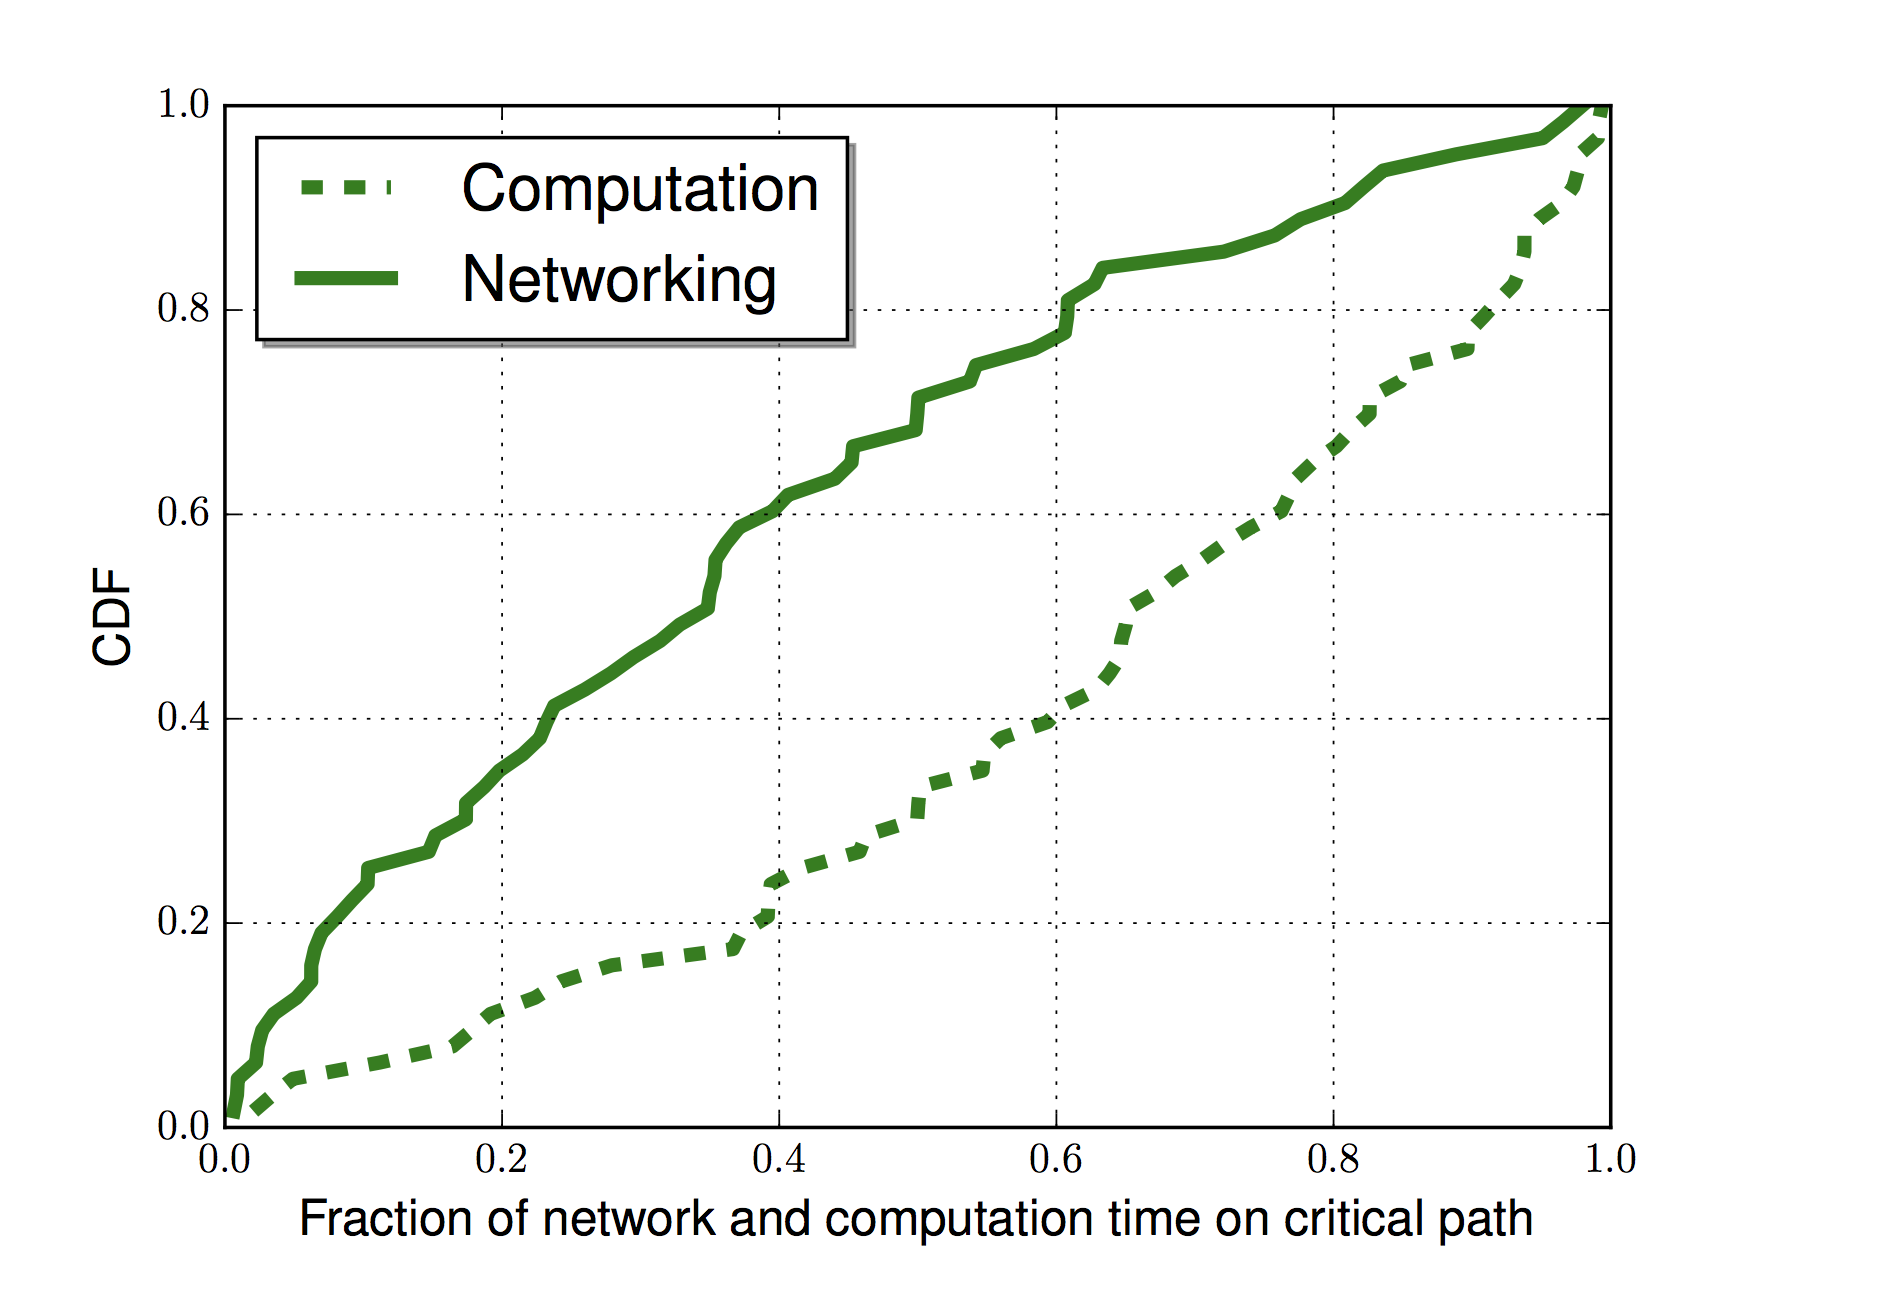
\includegraphics[width=0.9\columnwidth]{figs/comp_net.png}
\tightcaption{Runtime information on mobile devices}
\label{fig:mobile-runtime}
\end{figure}

\begin{figure}[t]
\centering
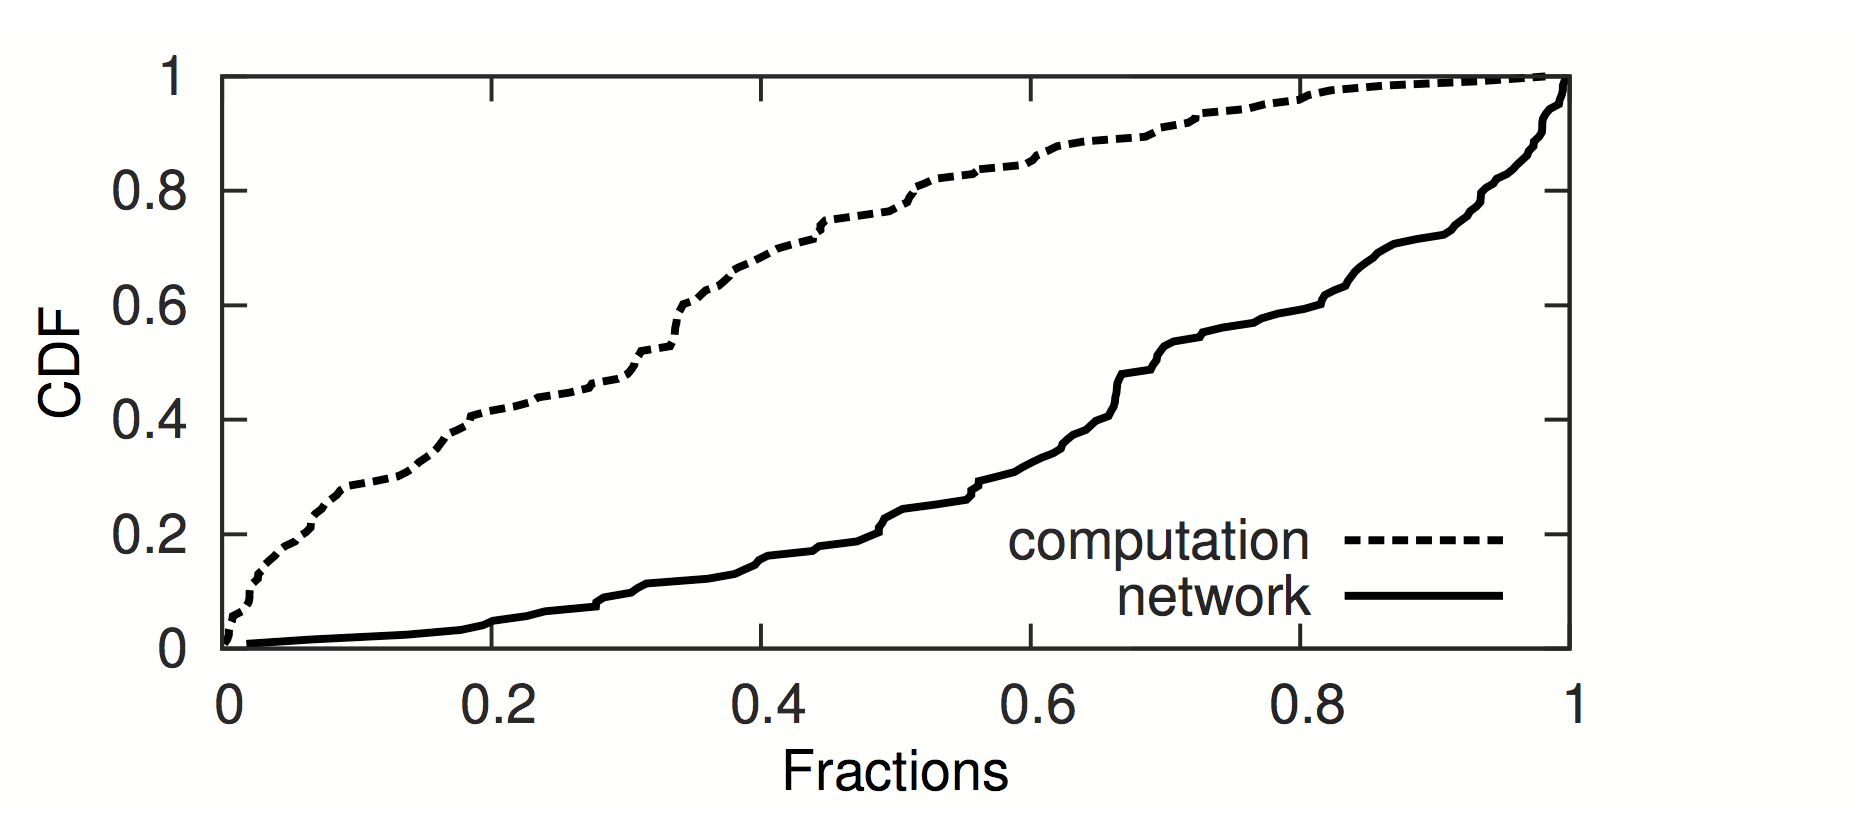
\includegraphics[width=0.9\columnwidth]{figs/comp_net_desk.png}
\tightcaption{Runtime information on desktops}
\label{fig:mobile-runtime}
\end{figure}

% \begin{figure}[t]
% \centering
% \begin{tabular}{cc}
% 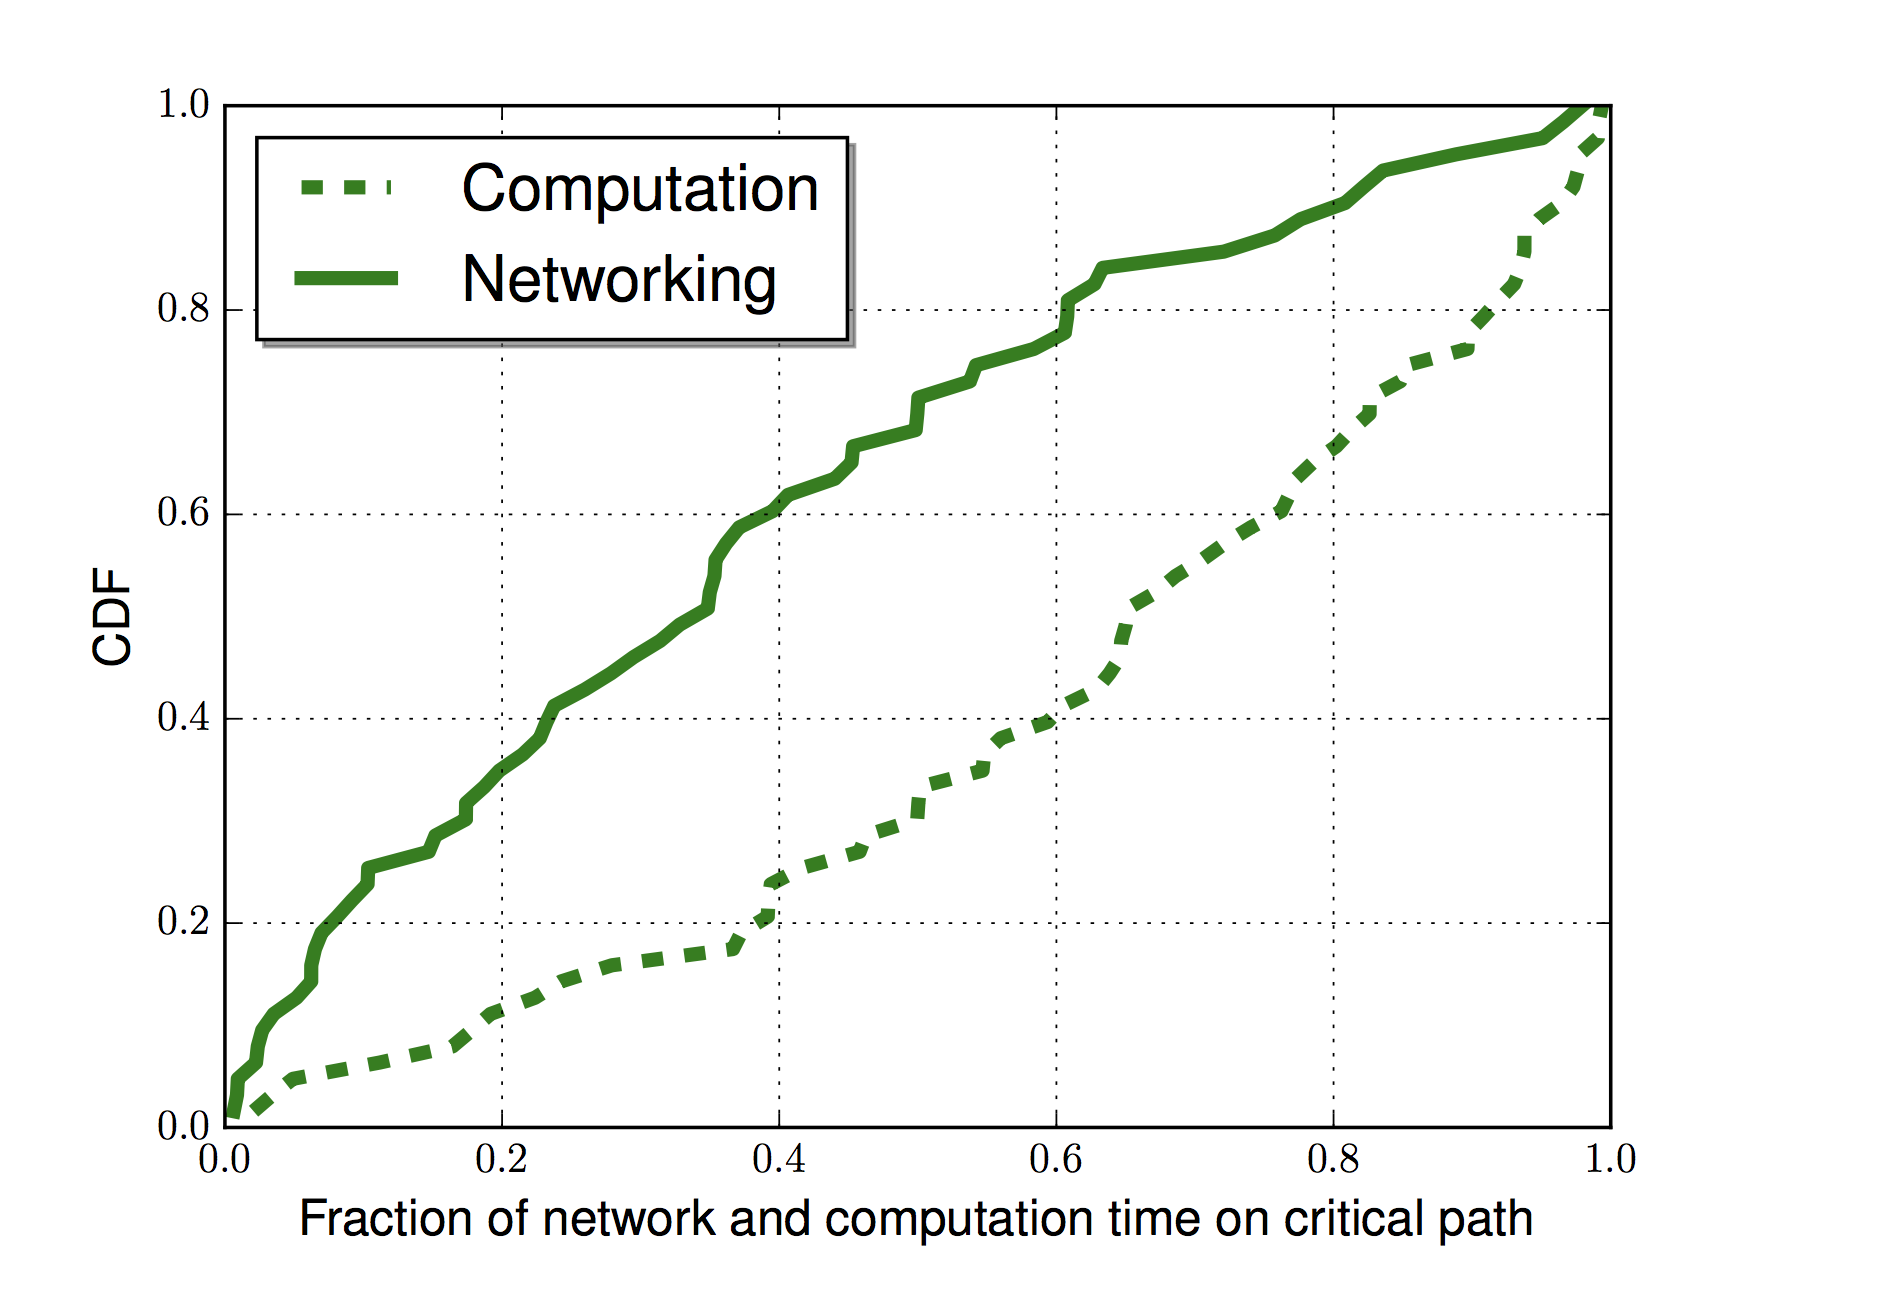
\includegraphics[width=0.9\columnwidth]{figs/comp_net.png}&
% 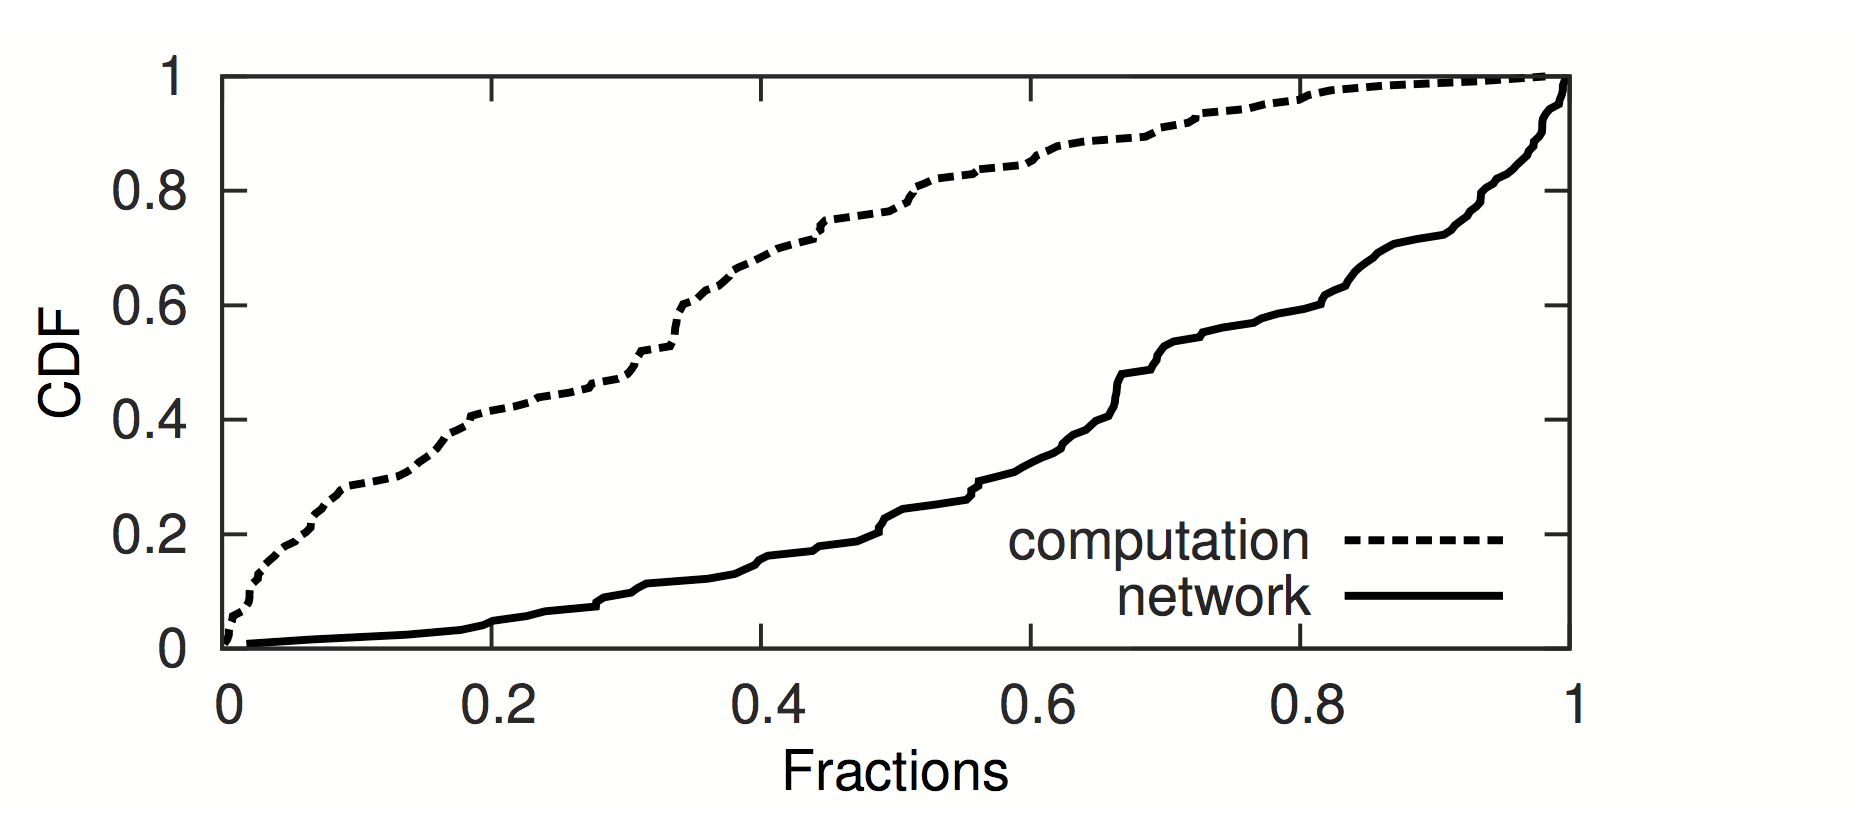
\includegraphics[width=0.9\columnwidth]{figs/comp_net_desk.png}\\
% {\small (a) Azure} & {\small (b) AWS}
% \end{tabular}
% \label{fig:dcs-local}
% \end{figure}

We propose a new technique to improve the page load time by reducing the Javascript execution time,
specifically the execution and script evaluation time.  
In order to do this, we intend to build a new caching framework for Google Chrome. We choose to focus on Chrome because it accounts for about 50\% of the market share in terms of browser
usage. Our caching framework will store the Javascript execution result. This can mean a lot of things
due to the dynamic nature of Javascript. Most of the time it is simply the return value of a 
Javascript function. At other times it can be a modified DOM structure or just an intermediate result which
will be further processed as input to other Javascript functions. 
We further define Javascript execution output in Section 3.1.

The expiry of our implemented Javascript execution cache will be the same as the expiry of the Javascript source cache.
The expiry is currently derived from the x-cache header field in the response, which determines how long
the Javascript source will reside in the browser cache. 
There are many caveats to this approach, such as coming up with an optimal data structure to hold the 
Javascript execution cache and handling non determinism of the Javascript code.
The biggest challenge when developing a new caching framework is modifying the massive code base of Google Chrome. However, Chrome already implements caching at the Javascript runtime level and we assume that much of this archicture can be borrowed
for the execution cache as well. 
Another potential challenge will be the memory overhead. Most popular websites run thousands of Javascript functions and caching the output of all 
of these functions will add an extra memory overhead to current browsers. 

\subsection{Javascript Execution Output}
\label{sec:exec-output}

The key idea for capturing a website's Javascript execution output 
is to capture the global changes made to the environment. This eliminates the need to capture any local computation, intermediate results computed, and any output
that does not affect the global state of the browser.We define the global state of the browser to be represented by the window object, which is
an instance of the open window/tab of the browser. This window object is supported by all the 
major browsers like Chrome, Firefox, Safari. 
If the execution of any javascript doesn't modify the window object in any way, then essentially
that javascript has no affect to the global browser window state and therefore has no impact.

 
Modification of the global window object can be either from modifications to the current properties of the window
object or the creation of new properties. Any global variable
and function that is defined by the javascript becomes a new property of the window object.

\subsection{Capturing JS Output}
\label{sec:exec-output}

Our system for evaluating the changes in Javascript execution will observe the changes in outputs from the following granularities:  
\squishenum
\item Website
\item Javascript file 
\item Javascript function
\squishenumend
We capture the entire window object state
before and after the page has loaded to observe global changes to the website. We then perform a diff of these
two window states to compare which properties have been modified during Javascript execution. This difference shows how much output must be cached and thus allows us to observe what the memory requirements for our caching framework will be.

We also capture the window object state after page loads across various time intervals to study how the global Javascript properties change over time. This data shows how much of the Javascript execution output can be cached and thus the impact caching can have on  
page load time. 

To the best of our understanding, if 95\% properties of the global window object remain unchanged across page loads, then we have a theoretical upper bound of a 95\% reduction in 
Javascript execution time by employing our caching framework. We conducted a series of experiments 
to understand how much change is made to the window object when the page is loaded after three seconds (Figure 3),
three hours (Figure 4) and three days (Figure 5). 
To our surprise, the change in the window object is extremely minimal, which leads us to expect a significant decrease in PLT
with our caching framework. 

However, Javascript files rarely contain single functions and thus to better understand the computation
effects of a Javascript file, we evaluate the execution output at the function level. 

To measure the effect of individual Javascript functions to the global state we create a call graph of the Javascript program during a page load. This dynamic call graph will be built during the page load. Each node
in the graph represents an invoked function. Each node contains a signature for the function that was executed. 
This signature contains the function name, arguments, any global variables,
and the return value. We use this signature to compare graphs across two different loads to 
establish how much of the execution can be cached. 


We plan to cache Javascript execution at a function level. The results from the above two studies
help us to define the upper bound of improved PLT with our caching framework. 
We have yet to implement this caching framework and evaluate the actual benefits of this approach.
